% *************************************************************************
% *    IWI Hamburg / Prof. Dr. Stefan Voß
% *    Thesis / Dissertation Latex Template                                        
% *    
% *    Author: Leonard Heilig <leonard.heilig@uni-hamburg.de>
% *   
% *    Note: some parts of this template are based on the VSIS template
% *              of Michael von Riegen <riegen@informatik.uni-hamburg.de>
% *   
% *************************************************************************

\documentclass[
      paper=a4,
      12pt,
      twoside=false,
      openright,
]{scrbook}



% DEFINE THESIS SETTINGS
% Bitte füllen Sie die folgenden Daten vollständig aus
\newcommand\myName{Max Mustermann}
\newcommand\myAddress{Musterstr. 7e, 22529 Hamburg}
\newcommand\myEmail{max.mustermann@studium.uni-hamburg.de}
\newcommand\myKeywords{<...>} % Optional
\newcommand\myMatNr{<...>}
\newcommand\myTitle{Titel}
\newcommand\myShortTitleForHeader{Kurztitel}
\newcommand\thesisType{<Expos\'{e} / Bachelorarbeit / Masterarbeit>}
\newcommand\faculty{<...>} % z.B. MIN-Fakultät
\newcommand\fachbereich{} % Optional: z.B. Fachbereich Informatik
\newcommand\courseOfStudies{<...>}
\newcommand\supervisor{<Name des Betreuers>}
\newcommand\primaryReferee{<Name des Erstgutachters>}
\newcommand\primaryRefereeInst{<Institute of Information Systems>}
\newcommand\secondaryReferee{<Name des Zweitgutachters>}
\newcommand\secondaryRefereeInst{<Name des Instituts>}
\newcommand\optionalQuote{} % shown after title page

\title{\mytitle}
\author{\myName \\ \texttt{\myEmail}}

% IMPORT PACKAGES AND SETTINGS
\usepackage{settings}





% ************ DOCUMENT BEGINS

\begin{document}

    % CHOOSE "ngerman" or "english"
    \selectlanguage{ngerman}
    
    % Please change this part to _titlepage_en for the English version
    % *************************************************************************
% *    IWI Hamburg / Prof. Dr. Stefan Voß
% *    Thesis / Dissertation Latex Template                                        
% *    
% *    Author: Leonard Heilig <leonard.heilig@uni-hamburg.de>
% *   
% *    Note: some parts of this template are based on the VSIS template
% *              of Michael von Riegen <riegen@informatik.uni-hamburg.de>
% *   
% *************************************************************************

\begin{titlepage}

% START PAGE: -1
\setcounter{page}{-1}    

\begin{figure}[h]
    
     \begin{flushleft}
     	
     \end{flushleft}
     \hspace{-40px}
     \noindent\begin{minipage}[t][0px][b]{0.3\textwidth}
     	%\noindent
\includegraphics[width=8cm,clip]{images/up-uhh-logo-u-2010-u-png}
     	\noindent
\includegraphics[scale=0.3]{images/UHH-Logo_2010_Farbe_CMYK.pdf}
     \end{minipage}
     \hspace{50px}
     \begin{flushright}
     	
     	\begin{minipage}[t][-70px][b]{0.38\textwidth}
     		\begin{flushright}
     			\sffamily{
     			%	{\small \textbf{Institute of Information Systems} } \\
     			%	\small Prof. Dr. Stefan Voß \\
     			}
     		\end{flushright}
     	\end{minipage}
     	\hspace{5px}
     	\begin{minipage}[t][-47px][b]{0.14\textwidth}
     	%	
\includegraphics[width=2cm,clip]{images/IWI_logo}
     	\end{minipage}
     \end{flushright}
     

    
\end{figure}

\vfill
\vspace{10mm}

\large
\begin{center}

    % THESIS TYPE
	\noindent { 
	 \color{uhhred}\textbf{\MakeUppercase \thesisType}
	}
	\vspace{2.0cm}\\
	% THESIS TITLE
	\textbf{\Large \myTitle} 
	\vspace{2.0cm}\\ presented by
\vspace{0.4cm}\\
\myName
	
\end{center}
	
\vfill

\begin{tabbing}
	\hspace{10em} \=  \kill
	%Presented by: \> \textbf{\myName} \\
	%\> \textrm{\myAddress} \\
	%\> \textrm{\myEmail} \\ 
	Faculty: \>  \faculty \\
	\> \fachbereich \\
	Course of Studies: \>  \courseOfStudies \\ %~(Semester \currentSemester)
	Matriculation Number: \>  \myMatNr \\ \\
	Supervisor: \> \supervisor \\
	Primary Referee: \> \primaryReferee \\
	 \>	\primaryRefereeInst \\
	Secondary Referee: \> \secondaryReferee \\
	 \>	\secondaryRefereeInst \\
	%Date of submission: \> \dateOfSubmission \\
\end{tabbing}


% BLANK PAGE WITH A QUOTE (OPTIONAL)
\newpage 
	
\thispagestyle{empty}
\setcounter{page}{0}

~\\ \vfill \noindent 
\optionalQuote

\end{titlepage}

\renewcommand{\cfttabpresnum}{Tab. } 
\renewcommand{\cftfigpresnum}{Fig. } 
\renewcommand{\nomname}{List of Abbreviations}
\renewcommand{\contentsname}{List of Contents}
\renewcommand{\listfigurename}{List of Figures}
\renewcommand{\listtablename}{List of Tables}


    \frontmatter  % ROMAN NUMBERING              
    %\textbf{Stichwörter :} \myKeywords
\subsubsection{Abstract}



	
    \tableofcontents
    
    \listoffigures
    \addcontentsline{toc}{chapter}{\listfigurename}
    
    \listoftables
    \addcontentsline{toc}{chapter}{\listtablename}
    

    % LIST OF ABBREVIATIONS
    \makenomenclature
    \printnomenclature[9em]

    \mainmatter % ARABIC NUMBERING            

    % INCLUDE TEX CHAPTERS
    \chapter{Einleitung}
Im Jahr 1956 wurde die erste Werbung im deutschen Fernsehen ausgestrahlt \cite{tagesspiegel_2016}. Mit ihrem Werbespot legte das Unternehmen \emph{Henkel} den Grundstein für eine Industrie, die Investitionen von 26,79 Milliarden Euro im Jahr 2018 rechtfertigt \cite{statista_werbung_2020}. Durch Innovationen wie das Internet und Smartphones verbringt laut \cite{statista_internetnutzung_2020} ein Großteil der Menschen in Deutschland heute viel Zeit im digitalen Raum und dementsprechend dringt auch Werbung in diesen ein. Für das automatisierte Vermitteln von Anzeigen kümmern sich sogenannte \emph{Ad-Broker}, die gleichzeitig auch als Zahlungskanal zwischen den involvierten Parteien fungieren. Also Folge dessen mangelt es dem Vergabeprozess an Transparenz und eine Provision wird von ihnen erhoben.\\

In den letzten Jahren haben Kryptowährungen eine erhöhte Aufmerksamkeit bekommen und gewinnen immer mehr an Akzeptanz, jedoch werden diese oft nur als spekulative Investitionsmöglichkeit betrachtet. Hinter ihnen verbirgt sich allerdings die sogenannte \emph{Blockchain-Technologie}, die als Lösung für Zahlung und Transparenz dienen könnte. Aufgrund ihrer Möglichkeiten stellt sich die Frage, inwieweit das Online Advertising vom heutigen Stand der Blockchain-Technologie profitieren kann.\\

Im Rahmen dieser Arbeit soll den Leser:innen ein Einblick in das Online Advertising verschafft werden. Die derzeitige Funktionsweise und Schwachpunkte des Systems sollen aufgezeigt werden, sodass mögliche Lösungsansätze mithilfe von Blockchain-Technologie gefunden werden können. Insbesondere soll den Leser:innen ein Verständnis über Blockchain-Technologie vermittelt werden, das über den Charakter einer rein spekulativen Investition hinausgeht.\\

Die Bachelorarbeit besteht aus drei Kapiteln. Im Ersten wird das derzeitige Finanzsystem thematisiert und sowie mögliche Vorteile von Blockchain-Technologie genannt. Im Anschluss wird die grundlegende Technologie am Beispiel von \emph{Bitcoin} erläutert. Das zweite Kapitel beschäftigt sich damit, wie \emph{Ethereum} bereits thematisierte Konzepte erweitert. Sobald ein ausreichendes Wissen über Blockchain-Technologie erreicht wurde, wird im dritten Kapitel das Online Advertising dargestellt und in Form eines Proof-of-Concept eine geeignete Webanwendung, welche Blockchain-Technologie verwendet, entwickelt. Den Schluss bilden eine Diskussion der Ergebnisse sowie Beantwortung der Leitfrage, eine Zusammenfassung der Kapitel und ein Ausblick, in dem mögliche kommende Innovationen genannt und alternative Anwendungsbeispiele genannt werden. 


    \chapter{Kapitel}

\section{Unterkapitel}

\subsection{Unterunterkapitel}

\lipsum[2]

\begin{figure}[h!]
	\centering
		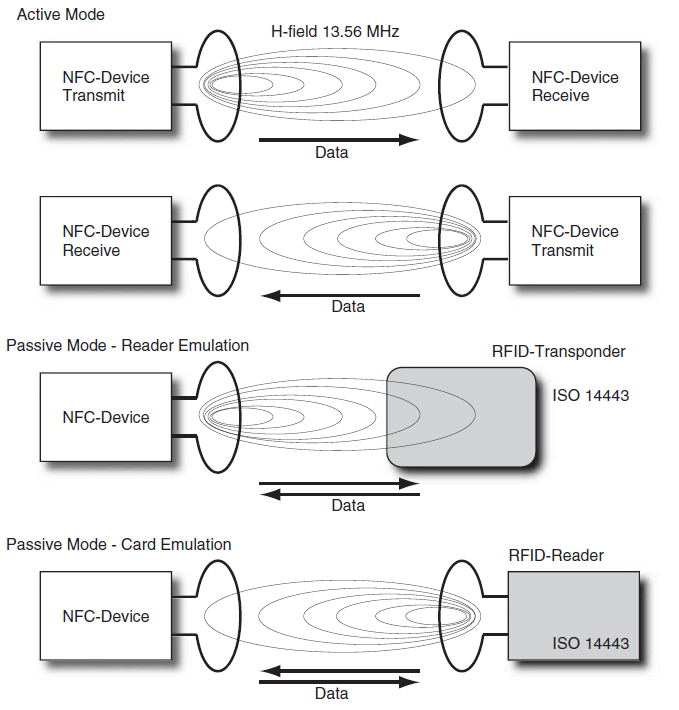
\includegraphics[width=0.6\textwidth]{images/nfc_communication}
		\vspace*{0pt}
	\caption[NFC operating modes]{NFC operating modes \citep[p.~58]{Finkenzeller.2010}}
	\label{fig:nfc_communication}
\end{figure}

\lipsum[2]

\begin{equation}
	\overline{x} = \frac 1n \sum^n_{i=1} x_i
\end{equation}

\lipsum[2] 

My reference to Tabelle~\ref{tbl:beispieltabelle1}.

% Zur Generierung von Tabellen kann das Excel-Plugin "Excel2Latex" verwendet werden
\begin{table}
	\centering
	
		\begin{tabular}{|l|l|r|}
		\hline
			\textbf{Farbe} & \textbf{Form} & \textbf{Zahl} \\
		\hline
			Rot & Rechteck & 100 \\
		\hline
			Blau & Kreis & 99 \\
		\hline
			Gelb & Dreieck & 98 \\
		\hline
		\end{tabular}
		\caption{Another table layout}
	    \label{tbl:beispieltabelle1}
	
\end{table}

\subsection{Unterunterkapitel 2}

\section{Unterkapitel 2}

\section{Unterkapitel 3}
    \chapter{Blockchain 2.0}
\section{Probleme von Bitcoin und Erweiterung der Konzepte durch Ethereum}
\section{Theoretische Grundlagen von Ethereum}
    \chapter{Blockchain im Online Advertising}
\section{Wie Online Advertising funktioniert}
\section{Mögliche Verbesserungen mittels Blockchain-Technologie}
\section{Programmierung eines geeigneten Smart Contracts in Solidity}
\section{Beantwortung der Forschungsfrage}
\section{Blockchain 3.0 - Bestehende Probleme und potenzielle Lösungen}
    \include{chapter05}
    \chapter{Schlussteil}
\section{Diskussion der Ergebnisse}
Durch die Nutzung von Blockchain-Technologie konnte ein direkter Zahlungskanal zwischen Besitzern der Webseiten und Unternehmen hergestellt werden. Dadurch wird das Schalten von Anzeigen für Besitzer solcher Webseiten profitabler. Gleichzeitig wird mehr Transparenz geschaffen, indem Unternehmen über eine Id direkt auf Metriken, die auf der öffentlichen Blockchain hinterlegt sind, zugreifen können. Somit haben sie einen vollen Einblick in die Situation ihrer Anzeige und können eine beliebige Anzahl an Metriken erfassen. Diese Lösung hat einen positiven Einfluss auf Besucher der Seite, denn ihre Daten werden nicht mehr verwendet und ist in diesem Aspekt datenschutzrechtlich vorzuziehen.\\

Die entwickelte Webanwendung entsprach zwar den Anforderungen zu Zahlungsfluss und Transparenz, weist jedoch gleichzeitig Schwachstellen in diesen Bereichen auf. Die Zahlung zwischen den beiden involvierten Parteien wurde zwar ohne eine Dritte Partei, welche als Zahlungskanal fungiert, ermöglicht, doch liegen, zum Zeitpunkt dieser Arbeit, die Kosten für eine Transaktion laut \cite{etherscan_2021} bei durchschnittlich 2,6 Dollar. Wenn man die Funktionen der Webanwendung betrachtet, stellt dies ein Problem beim Schalten der Anzeigen dar, denn dort wird jedes Mal der Zähler für die Anzeige in der Blockchain erhöht. Jeder Funktionsaufruf im Smart-Contract wird durch eine dementsprechend teure Transaktion ausgelöst. Jede zusätzliche Metrik muss verfolgt werden, sodass die laufenden Kosten für die Internetseite in keinem Verhältnis zum Wert der Impressionen steht.
Die geschaffene Transparenz bringt ebenfalls Nachteile mit sich, denn es kann sich jede Person, mithilfe der Id, Zugriff auf die Metriken von Anzeigen verschaffen. Dies ist aus Sicht der Unternehmen, die miteinander konkurrieren, unvorteilhaft. Zusätzlich zu den genannten Schwachpunkten, verlieren die involvierten Parteien Vorteile des Programmatic Advertising. Durch Verwendung der Blockchain muss die Partei, welche den Werbeplatz zur Verfügung stellt, einen hohen Aufwand betreiben, um die gesamte Infrastruktur bereitzustellen. Im Vergleich dazu, reicht beim Programmatic Advertising das Einfügen eines Code-Snippets in den Quellcode der eigenen Internetseite, was deutlich weniger Programmierkenntnisse erfordert. Den Unternehmen entgeht der Vorteil, dass ihre Anzeigen vollautomatisiert relevante Kundensegmente erreichen.\\

Nach Betrachtung der Ergebnisse kann angenommen werden, dass Online Advertising nicht sonderlich von dem jetzigen Stand der Blockchain-Technologie unter Ethereum profitieren kann.
\section{Zusammenfassung}
Begonnen hat die Arbeit mit der Einleitung...\\
 
Anschließend wurde Blockchain-Technologie am Beispiel von Bitcoin erläutert. Dafür musste allerdings zunächst die Funktionsweise und technische Anforderungen von klassischem Geld untersucht werden, sodass ein Bezug zu Kryptowährung, die auf Blockchain-Technologie basiert, und ihrer Eignung hergestellt werden konnte. 
Danach wurde die Theorie hinter der Blockchain-Technologie am Beispiel von Bitcoin erläutert. 
Das Unterkapitel \emph{Keys und Adressen} folgte dem Weg von der Erzeugung des privaten Schlüssels, welcher Besitzer zum signieren von Transaktionen autorisiert, bis hin zur Generierung von Adressen, mit denen Guthaben empfangen werden kann. 
Daran anknüpfend wurde die Funktionsweise des SHA256-Algorithmus, welcher an verschiedenen Stellen des Bitcoin-Protokolls verwendet wird, nach \cite{dang_2015} erläutert. 
Verglichen wurden anschließend 2 verschiedene Arten von Wallets, die zur Verwaltung von Schlüsseln verwendet werden.
Darauf folgte die Erklärung zu Transaktionen im Bitcoin-Protokoll, die das Prinzip der \emph{Unspent Transaction Outputs} und Transaktionskosten umfasste.
Welche Akteure es im Bitcoin-Protokoll gibt, als auch das Hinzufügen neuer Teilnehmer, wurde in \emph{Die verschiedenen Akteure im Netzwerk} besprochen.
Anschließend folgte das eigentliche Kernthema, die \emph{Blockchain} sowie der Weg, den eine Transaktion bewältigt, bis sie Teil der Blockchain ist. Zum Schluss wird kurz beschrieben, wieso ein Angriff auf das Netzwerk nicht wahrscheinlich ist.\\

Im Kapitel \emph{Blockchain 2.0} wurde das Ethereum-Protokoll näher untersucht. Es wurden Neuerungen im Vergleich zu Bitcoin aufgezeigt, wie andere Mechanismen bei den Transaktionen oder auch der Verbrauch von \emph{Gas}.
Um das neue Konzept der \emph{Smart-Contracts} näher zu untersuchen, wurde zunächst erläutert, wie die \emph{Ethereum Virtual Machine} Anweisungen, die sie in Form von Transaktionen erhält und anhand dieser den Zustand der Blockchain verändert. Daraufhin wurde die Syntax der Programmiersprache \emph{Solidity} aufgezeigt und mit Konzepten gängiger Programmiersprachen verglichen.
Zum Schluss wurden kurz mögliche Use-Cases für den Einsatz von Smart-Contracts genannt.\\

Nachdem ein ausreichender Wissensstand zur Blockchain-Technologie erreicht wurde, beschrieb das Kapitel \emph{Blockchain im Online Advertising} den Kontext der gleichnamigen Industrie. Genauer wurde auf das Thema \emph{Display Advertising} eingegangen und wie heutzutage \emph{Programmatic Advertising} dort Verwendung findet. Die Funktionsweise, sowie Stärken und Schwächen wurden aufgezeigt und anschließend mögliche Verbesserungen mittels Blockchain-Technologie genannt. Im Anschluss daran wurden die Ideen in Form eines Proof-of-Concept umgesetzt und die einzelnen Komponenten, sowie relevanter Programmcode näher erläutert.\\

Es konnte zwar eine funktionsfähige Anwendung entwickelt werden, doch weist diese in anderen Aspekten gravierende Mängel auf, sodass Entschluss gefasst wurde, dass Blockchain-Technologie auf ihrem jetzigen Stand keine Vorteile bietet, die zu einer ernsthaften Alternative zum Programmatic Advertising macht.
\section{Ausblick}
Im Rahmen dieser Arbeit wurden die beiden größten Kryptowährungen Bitcoin und Ethereum näher untersucht, doch sind diese bei Weitem nicht die Einzigen. Rund um das Thema Kryptowährungen hat sich laut \cite{coinmarketcap_2021} eine Industrie mit einer Marktkapitalisierung von derzeit mehr als einer Billion US-Dollar gebildet (Stand Mai 2021). Sogar große US-Banken wie Goldman Sachs nehmen mittlerweile Kryptowährungen wahr, sodass in dieser Industrie weitere Innovationen zu erwarten sind \cite{handelsblatt_2021}. Dies könnten Innovationen wie die Verwendung von Proof-of-Stake statt Proof-of-Work, welches von der Cardano-Plattform verwendet wird und im Paper \cite{kiayias_2019} untersucht wird, zur Folge haben. Damit stellt vor dem Hintergrund der Klimaerwärmung eine vorteilhafte Alternative zum ressourcen-intensiven Proof-of-Work dar. Genauso könnte das Problem der Skalierbarkeit in Zukunft gelöst werden, um günstigere Transaktionen ohne Verlust der Dezentralisierung ermöglichen zu können.\\

Sobald dadurch günstigere Transaktionen ermöglicht werden, könnten weitere Möglichkeiten von Blockchain-Technologie im Online Advertising untersucht werden. Beispielsweise wird in \cite{ding_2021} ein System vorgestellt, welches, genau wie der Proof-of-Concept dieser Arbeit, Blockchain-Technologie für die Zahlung von Unternehmen, die Werbeflächen für ihre Anzeigen erwerben möchten, verwendet. Zusätzlich dazu wird darin beschrieben, wie man die Nutzer, welche der Werbung ausgesetzt sind, entlohnen könnte. Das Unternehmen \emph{Brave} verfolgt mit ihrem gleichnamigen Browser, welcher einen Ad-Blocker enthält, ein ähnliches Ziel. Nutzer können ihre Zustimmung dafür geben, dass sie dafür entlohnt werden, Werbung, die vom Browser in Form einer Push-Benachrichtigung angezeigt werden, zu erhalten. Mithilfe eines Voting-Systems könnte man Nutzer Anzeigen bewerten lassen, um so, ohne das Sammeln von Daten, wie es beim Programmatic Advertising nötig ist, nur relevante Anzeigen schalten zu können. Dafür würden sie dann anschließend für ihre Aufmerksamkeit eine Entlohnung erhalten. Statt der Sammlung ihrer Daten könnten die Nutzer, welche den Anzeigen ausgesetzt sind, somit am Wertschöpfungsprozess beteiligt werden.



    
\appendix
\chapter{Anhang}
Lorem ipsum dolor sit amet, consectetuer adipiscing elit. Cras semper. Integer sapien nulla, consectetuer a, laoreet et, varius quis, mauris. Nunc pharetra tincidunt massa. Pellentesque habitant morbi tristique senectus et netus et malesuada fames ac turpis egestas. Praesent pellentesque mauris at elit. Aliquam consequat suscipit enim. Pellentesque habitant morbi tristique senectus et netus et malesuada fames ac turpis egestas. Nunc sapien. Proin hendrerit diam at quam. Lorem ipsum dolor sit amet, consectetuer adipiscing elit. Integer vulputate semper nunc. Sed dui. Praesent at sem. Integer elit ipsum, placerat vitae, dictum quis, feugiat sit amet, metus.

\section{Anhang A}
Donec arcu turpis, pretium quis, interdum non, condimentum a, est. Fusce lobortis urna non tellus. Nam leo dui, malesuada non, tempus placerat, congue eget, pede. Mauris porttitor risus quis tortor molestie vehicula. Curabitur tincidunt. In malesuada congue nisi. Nullam et nulla. Curabitur porttitor. Ut molestie sagittis felis. Sed urna libero, ultricies quis, laoreet eget, congue id, metus. Proin ac lorem cursus mauris auctor laoreet. Donec justo. Etiam nunc sem, dapibus sit amet, euismod a, molestie sit amet, mi.

Morbi sollicitudin consequat magna. Vivamus dictum. Nulla non quam. Nam sem tellus, aliquam sed, hendrerit nec, imperdiet ut, augue. Aliquam erat volutpat. Vivamus non ligula sit amet lorem accumsan viverra. Cras mattis libero et ante. Cras massa. Donec fringilla, metus vitae semper condimentum, dolor dui fringilla arcu, et mattis nulla dui vel lectus. Nunc mauris magna, tristique eu, rutrum at, facilisis eu, odio. Nullam congue magna non nisi. Suspendisse viverra, massa non pellentesque scelerisque, risus elit 

\noindent Hier kommt ein Listing \ref{lst:soap}.

\begin{center}
\begin{lstlisting}[caption={SOAP Anfrage an einen HalloWelt-Web-Service},captionpos=b,language=XML,label={lst:soap}]
<?xml version='1.0' encoding='UTF-8'>
<SOAP-ENV:Envelope (*@\label{lst:soapEnv}@*)
  xmlns:SOAP-ENV="http://schemas.xmlsoap.org/soap/envelope/"
  xmlns:xsi="http://www.w3.org/2001/XMLSchema-instance"
  xmlns:xsd="http://www.w3.org/2001/XMLSchema"
  xmlns:ns1="http://localhost/wsdl/HalloWeltService.wsdl">
  
  <SOAP-ENV:Body>(*@\label{lst:soapBody}@*)
  	<ns1:gruss>
  		<name xsi:type="xsd:string">
  			Michael
  		</name>
  	</ns1:gruss>
  </SOAP-ENV:Body>

</SOAP-ENV:Envelope>
\end{lstlisting}
\end{center}

bibendum dolor, vitae ultrices lorem neque et erat. Nullam tortor ante, venenatis et, aliquet ac, ornare id, massa. Vivamus urna augue, posuere vitae, sagittis id, porttitor at, arcu. Praesent pharetra rutrum neque. Maecenas tempor ultrices felis.
Nulla facilisi. In sed elit aliquet neque malesuada blandit. Nam tempus imperdiet eros. Mauris tincidunt diam eu erat. Phasellus iaculis blandit leo. Nunc augue. Donec dignissim accumsan pede. Ut consequat, eros id accumsan placerat, mi justo ullamcorper pede, id lacinia augue nisi non nibh. Vestibulum eget arcu. Cras pretium, dui eu gravida varius, lectus neque accumsan ligula, eu sodales magna lectus ut nisi. Aliquam vel ante. Ut suscipit porta augue. Suspendisse pellentesque faucibus nisl. Nulla magna tortor, cursus quis, varius quis, hendrerit ut, neque.


    \cleardoublepage
    
    \urlstyle{same}
    \bibliographystyle{chicagog}
    \begingroup
    \interlinepenalty=10000
    \hyphenpenalty=105000
    \exhyphenpenalty=105000
   
   \addcontentsline{toc}{chapter}{Bibliography}
    \bibliography{thesis}
    \endgroup
    \cleardoublepage

    % Please DO NOT change the declaration (even it is in German)
    % *************************************************************************
% *    IWI Hamburg / Prof. Dr. Stefan Voß
% *    Thesis / Dissertation Latex Template                                        
% *    
% *    Author: Leonard Heilig <leonard.heilig@uni-hamburg.de>
% *   
% *    Note: some parts of this template are based on the VSIS template
% *              of Michael von Riegen <riegen@informatik.uni-hamburg.de>
% *   
% *************************************************************************
\chapter*{Eidesstattliche Versicherung}

\thispagestyle{empty}
\addcontentsline{toc}{chapter}{Eidesstattliche Versicherung}

Hiermit versichere ich an Eides statt, dass ich die vorliegende Arbeit im Studiengang \courseOfStudies ~selbstständig verfasst und keine anderen als die angegebenen Hilfsmittel -- insbesondere keine im Quellenverzeichnis nicht benannten Internet-Quellen – benutzt habe. Alle Stellen, die wörtlich oder sinngemäß aus Veröffentlichungen entnommen wurden, sind als solche kenntlich gemacht. Ich versichere weiterhin, dass ich die Arbeit vorher nicht in einem anderen Prüfungsverfahren eingereicht habe und die eingereichte schriftliche Fassung der auf dem elektronischen Speichermedium entspricht.


\vspace{1.5cm} 

\noindent Hamburg, den \uline{~~~~~~~~~~~~~~~~~~~~~~~~~~~~~~~~~~~~~~~~~~~}~~~~~~~~~~~
~~Unterschrift: \uline{~~~~~~~~~~~~~~~~~~~~~~~~~~~~~~~~~~~~~~~~~~~~~~~~~~~} 


\cleardoublepage

\newpage

% empty page
\begin{titlepage}
\mbox{}
\end{titlepage}

\end{document}

